%%%%%%%%%%%%%%%%%%% Kapitel 5. %%%%%%%%%%%%%%%%%%%%%%%%%%%%%%

\chapter[Quäkerischen Weltmission]{Quäkerischen Weltmission}

\begin{center}
\textbf{Christus in uns. Erkenntnis der Quäkerischen Weltmission. Das
Haus Richter Fells in Swarthmore; der Pöbel 
von Ulverstone\ort{Ulverstone}.
Rechtfertigung vor dem Gericht in Lancastre.}
\end{center}



\begin{floatingfigure}[3]{4cm}
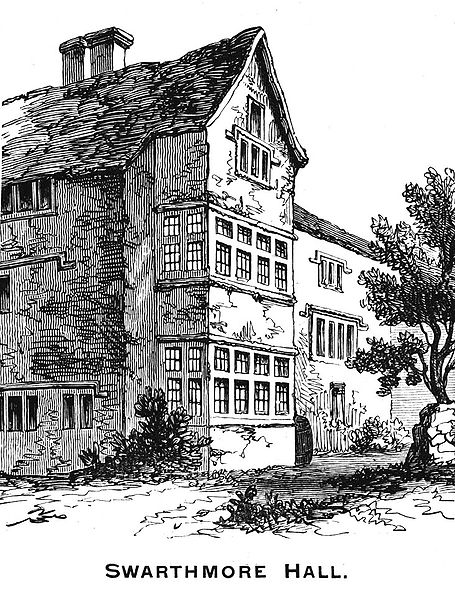
\includegraphics[width=0.20\textwidth]{./pics/swarthmore_hall.png}
\label{bild:swarthmoor} 
\end{floatingfigure}

\section{Kampf gegen Verleumdung}

Wir zogen durch Nottinghamshire\ort{Nottinghamshire} 
nach Lincolnshire\ort{Lincolnshire} [...].
Hier kam zu einer unserer Versammlungen ein Mann und erhob eine
falsche Anklage gegen mich; er verbreitete 
überall das Gerücht\index{Gerücht}, ich
habe gesagt, ich sei Christus, was gänzlich falsch war. Als ich dann
nach Gainsborough\ort{Gainsborough} kam, wo einer 
der Freunde auf dem Marktplatz die Wahrheit 
verkündet hatte, fand ich die ganze Stadt und
alle Marktleute in Aufruhr. Ich ging ins Haus eines Freundes,
und das Volk drängte sich hinter mir drein, bis das Haus ganz
voll war von \textit{Frommen}, Eiferern und Pöbel; da kam jener
falsche Verleumder herein und klagte mich öffentlich vor allen an,
ich hätte gesagt, ich sei Christus, und er habe Zeugen, es zu 
beweisen. Das brachte die Leute so in Wut, das man Mühe hatte,
mich vor ihnen zu schützen. Da trieb mich der Geist des Herrn
aus einen Tisch zu stehen und in der ewigen Kraft des Herrn
den Leuten zu verkünden, das Christus in ihnen sei, es sei denn,
das sie Verdammte seien; und das es Christus, die ewige Kraft
Gottes sei, welche jetzt aus mir zu ihnen rede, nicht ich sei Christus;
die Leute waren im allgemeinen befriedigt außer jenem \textit{Frommen}
und einigen falschen Zeugen. Ich nannte diesen Ankläger
Judas\index{Beleidigung}\index{Judas}\person{Fox!verbaler Angriff},
und es trieb mich, ihm zu sagen, das das Ende des Judas auch
das seine sein werde; solches lasse ihm der Herr durch mich sagen.


Des Herrn Macht kam über alle und beruhigte die Gemüter der
Leute und sie gingen in Frieden fort. Jener Judas aber machte
sich davon und erhängte sich und man steckte einen Pfahl in sein
Grab. Daraufhin erhoben die bösen 
Priester eine Verleumdung\index{Verleumdung}
gegen uns und streuten aus, ein Quäker habe sich erhängt in
Lineolnshire. Diese Lüge ließen sie drucken und verbreiten und
häuften so Sünde auf Sünde. Aber wir und die Wahrheit wurden
nicht davon getroffen; denn jener war so wenig ein Quäker als
der Priester, der solches gedruckt hatte; vielmehr war es einer
% \picinclude{./050-059/p_s057.jpg} 
ihrer eigenen Leute. Aber trotz dieser argen Lüge, mit welcher der
Gegner beabsichtigt hatte, uns zu verleumden und die Leute von
der von uns verkündeten Wahrheit abzukehren, nahmen doch viele
in Lincolnshire das Evangelium an, da sie von der ewigen 
Wahrheit überzeugt waren und sich zu Füßen des himmlischen Herrn
setzten [...].

\section{Schwere Misshandlung von Fox und Freunden}

Wir zogen nun wieder [...] über Warmsworth [...] Bably,
Doncaster [...] nach Tikhill, wo an einem Ersten Tage die
Freunde der Gegend sich versammelten, und es herrschte durch
Gottes Macht eine tiefe Zerknirschung in der Versammlung.
Ich verließ die Versammlung, da Gott mich trieb ins Turmhaus
zu gehen. Als ich dorthin kam, fand ich den Priester und fast
alle Gemeindeältesten im Chor beisammen. Ich ging zu ihnen
und hub an zu ihnen zu reden, aber sie fielen sogleich über mich
her, und ein Priester nahm seine Bibel und schlug mich damit
ins Gesicht, so das ich heftig blutete im Turmhaus; das Volk
schrie: \zitat{Hinaus mit ihm aus der Kirche!} Und als sie mich hinaus
gebracht hatten, prügelten sie mich und warfen mich zu Boden
und über eine Hecke; hernach schleppten sie mich durch ein Haus
auf die Straße; sie bewarfen mich mit Steinen und schlugen mich,
während sie mich Vorwärts rissen, so das ich über und über mit
Kot beschmiert war. Sie nahmen mir den Hut, den ich nicht
mehr wieder bekam. 

Als ich jedoch wieder auf den Füßen war,
verkündete ich ihnen das Wort des Lebens und zeigte ihnen, 
wohin ihre Lehre sie führe und wie sie das Christentum entehrten. Nach
einer Weile ging ich wieder in die Versammlung zurück zu den
Freunden. Und als die Priester und die Leute am Hause vorbei
kamen, ging ich mit einigen Freunden hinaus in den Hof und
redete zum Priester und den Leuten. Der Priester verhöhnte
uns und nannte uns \zitat{Quäker}. Aber die Macht des Herrn
kam dermaßen über sie und das Wort des Lebens wurde ihnen
so überzeugend und eindringlich verkündet, das der Priester selber
zu zittern\index{zittern} begann und einer 
sagte: \zitat{seht wie der Priester zittert
und bebt, er wird auch ein Quäker}. Als die Versammlung zu
Ende war, gingen die Freunde fort, und ich ging, ohne Hut,
nach Balby, etwa sieben bis acht Meilen weit. 

Die Freunde
wurden an dem Tage dergestalt von dem Priester und seinen
Anhängern misshandelt, das einige Friedensrichter, als sie davon
hörten, kamen und ein Verhör in dieser Stadt anstellten, um
% \picinclude{./050-059/p_s058.jpg} 
die Sache zu untersuchen. Der, welcher mich blutig geschlagen
hatte, fürchtete, man haue ihm die Hand ab; aber ich vergab
ihm und klagte nicht gegen ihn.

\section{}

Zu Anfang des Jahres- 1652 regte sich heftiger Widerstand
gegen die Wahrheit und die Freunde, bei Priestern und Volk
und bei etlichen der Behörden in Yorkshire, so das der Priester
von Warmöworth sich einen Verhaftbefehl gegen mich und Thomas
Aldam verschaffte, der in allen Teilen im westlichen Bezirk York-
shireö auögeführt werden konnte. Zu dieser Zeit hatte ich ein
Gesicht von einem Bären und zwei grosen, riesigen Hunden, und
wie ich bei ihnen vorbei muste, ohne das sie mir ein-as tun
konnten. Und so geschah es; denn der Konstabler ergriff Thomas
Aldam und brachte ihn nach York; und ich ging ein groseö Stück
Wegs mit ihm. Der Kanstabler hatte auch einen Verhaftbesehl
gegen mich und sagte zu mir: er sehe mich schon, aber er möge
nicht einen der ihm fremd sei, behelligen; Thomas Aldam sei
eben sein Nachbar. Also hielt ihn die Kraft des Herrn, das er
mich in Ruhe lies. Wir kamen in die Wohnung deö Leutnant
Roper, wo wir eine grose Versammlung hatten, worunter viele
angesehene Leute waren; die Wahrheit wurde mächtig kund
unter ihnen und die Schrift herrlich erklärt, und die Gleichnisse
und Reden Jesu wurden ausgelegt und die Kirche, wie sie in den
Tagen der Apostel war, und der Abfall von derselben. Die
Wahrheit gelangte zur Herrschaft an jenem Tage, so das jene
angesehenen Leute alle zugestanden: ,,diese Anschauungen werden
sich über die ganze Erde aus-breiten«. Dieser Versammlung
wohnten auch Jametz Naylor, Thomas Goodyear und William
Dewsbury, die das Jahr vorher gewonnen worden waren, sowie
Richard Farne-worth bei. Der Konstabler blieb mit Thomas
Aldam, bis die Versammlung auö war, darm ging er mit ihm
nach dem Gefängnis in York; mich aber lies er in Ruhe ....
Darnach kam ich nach Hightown, wo eine Fran wohnte, die
kurz vorher bekehrt worden war. Wir gingen in ihr Haus und.
hielten eine Versammlung, und die Leute versammelten sich, und
wir verkiindeten ihnen die Wahrheit und wirkten für den Herrn
unter ihnen, und sie gingen in Frieden wieder von dannen.
Aber ez war dort eine Witwe, namens Green, von böser Ge-
sinnung; diese ging zu einem sogenannten ,,Herrn« (cieutleman)
und verklagte unö bei ihm, obwohl er kein Beamter war. Am


% \picinclude{./050-059/p_s059.jpg} 
Christus in uns. Erkenntnis der Quäkerischen Weltmission usw. 59
nächsten Morgen sandten wir dem Priester einige Fragen. Alö
wir gerade fort gehen wollten, kamen einige, die sich zu une
hielten, gerannt und sagten, dieser Mörder habe sein Schwert
für uns geschärst und komme mit demselben gegen uns. Da wir
gerade fort gingen, oerfehlten wir ihn. Aber kaum waren wir
sort, so kam er in das Haus, in dem wir gewesen waren, und
es hies allgemein, wenn wir nicht fort gewesen wären, so wären
wir ermordet worden. Wir brachten die Nacht im Walde zu
und wurden ganz durchnäst, denn es regnete stark. Am Morgen
trieb es- mich roicher in die Stadt zurück, wo sie uns ausfiihrlich
über jenen Bösewicht berichteten.
Von da gingen wir nach Vradsord, wo wir Richard Farns-
worth trafen, von dem wir unö kurz vorher getrennt hatten.
A18 wir in sein Haus kamen, setzte man uns Fleisch nor, aber als
. ich anfangen wollte, geschah das Wort deö Herrn an mich: »Js nicht
Brot bei einem Neidischen« (Spr. 23, 6). Sogleich stand ich
vom Tische auf und as nicht;3. Die Frau war eine Baptistin.
Nachdem ich die ganze Familie ermahnt hatte, sich zum Herrn
zu bekehren und auf seine Lehre in ihren Herzen zu merken,
gingen wir von dannen ......
Unterwegs; kamen wir zu einem grosen Hügel, genannt Pend-
lehill; und der Herr trieb mich, aus denselben hinauf zu gehen,
mas ich mit groser Anstrengung tat, denn er war sehr steil und
hoch. Alö ich oben ankam, blickte ich auf das Meer, das Lan-
cashire umspült. Von diesem Hügel aut:-’ zeigte mir der Herr
die Orte, wo ihm ein grosetz Volk sollte gesammelt werden.
Beim Hinuntergehen sand ich eine Wasserquelle am Abhang
dez Hiigels, aus der ich mich ersrischte, denn ich hatte in den
letzten Tagen nur wenig gegessen und getrunken. Am Abend
kamen wir zu einer Herberge .... und hier lies mich der
Herr ein Gesicht sehen: eine grose Schar in weisen Kleidern
am Ufer eines Flusses, die zum Herrn kamen, und der Ort, den
ich sah, war bei Wen?-leydale und Sedbergh. . .
Wir zogen durch die Daleö . . . nach Dent .... Hier ging
ich zu Richard Robinson und redete von der Wahrheit zu ihm:
Ju einer Versammlung bei Frieden?-richter Benson traf ich Leute,
die sich vom öffentlichen Gotteödienst lozgesagt hatten. Dies
war der Ort, den ich gesehen, wo eine Schar in weisen Kleidern
daher kam. GS war eine grose Versammlung, und die meisten


% \picinclude{./060-069/p_s060.jpg} 
wurden gewonnen und haben noch jetzt grose Versammlungen von
Freunden in der Nähe von Sedbergh, die ich damals zuerst zu-
sammen sammelte im Namen Jesu.
GS fand ein groser Jahrmarkt statt, an welchem man pflegte
Dienstboten zu dingen; ich verkündete den Tag dee Herrn. Nach-
dem ich dietz getan, ging ich auf den Platz des Turmhausetz, und
viele Leute kamen vom Jahrmarkt zu mir und eine Menge Priester
und »Fwmme«. Da verkündete ich die ewige Wahrheit dez
Herrn und das Wort dez Lebenö während mehrerer Stunden
und zeigte, das der Herr gekommen sei, sein Volk selbst zu lehren
und es abzubringen von den Wegen dieser Welt und ihren Lehrern,
zu Ehristuö dem wahren Lehrer und wahren Weg. Jch machte
ihnen klar, wie ihre Lehrer denen gleich seien, die von jeher
von den Propheten, von Ehristus und den Aposteln verdammt.
worden sind. Jch ermahnte alle von ihren mit Händen gemachten
Tempeln abzulassen und auf den Empfang dez Geistes zu warten,
damit sie erkennen könnten, das sie der Tempel Gottes seien.
Nicht ein einziger von den Priestern hatte Macht, seinen Mund
auszutun gegen das, was ich verkündete; zuletzt sagte einer von
der Wache: ,,Warum geht ihr nicht in die ,,Kirche«? hier ist
kein geeigneter Platz zum Predigen«. Jch sagte ihm, ich leugne
ihre Kirche. Da erhob sich Francis Howgill,1) Prediger einer
Gemeinschaft. Er hatte mich nie vorher gesehen, aber er unternahm
es, diesem Hauptmann zu antworten und brachte ihn bald zum
Schweigen; und von mir sagte er: ,,dieser predigt gewaltig und
nicht wie die Schriftgelehrten (Matth. 7, 29)«. Jch erklärte da-
rauf den Leuten, das dieser Boden hier nicht heiliger sei alö an
einem andern Ort und das nicht dieses Haus die Kirche sei,
sondern die Gemeinde, deren Haupt Christutz ist. Bald nachher
kamen dann einige Priester zu mir und ich ermahnte sie, Buse zu
tun. Einer von ihnen sagte, ichsei verrückt, und wandte sich von
mir ab; aber manche wurden gewonnen an dem Tage und freuten
sich über die Verkündigung der Wahrheit und nahmen sie mit
Freuden auf. Einer unter ihnen, Hauptmann Ward, nahm die
Wahrheit in Liebe auf und lebte darin bis zu seinem Tode.. . .
Von da ging ich nach Unterbarrow, zu einem namens Miles
Bateman ..... Am Morgen ging ich aus . . und als ich in
1) Franeiö Hotogill, später ein eisriger Qnäkerprediger (s.Wein-
garten a. a. O.)


% \picinclude{./060-069/p_s061.jpg} 
Christns in uns. Erkenntnis der Quäkerischen Weltmission usw. 61
der Nähe auf einem Hügel hin und her ging, sah ich einige
Reisende, welche um Unterstützung baten, und ich sah, das sie
es nötig hatten; aber man gab ihnen nichts und sagte ihnen, sie
seien—Strolche. GS betrübte mich solche Hartherzigkeit unter den
,,Frommen« zu sehen, und ale sie alle beim Frühstück sasen, lies
ich den Reisenden etwa eine Viertelmeile nach und gab ihnen
etwas Geld. A16 nun einige von den andern aus dem Hause
kamen und sahen, das ich eine Viertelmeile weg war, sagten sie, ich
hätte nicht so weit kommen können, wenn ich nicht Flügel hätte.
Daraufhin war es nahe daran, das man die Versammlung ab-
sagte; denn man hatte eine so merkwürdige Meinung von mir
bekommen, das viele nicht eine Versammlung mit mir haben
wollten. Jch sagte ihnen, ich sei jenen armen Reisenden nachge-
laufen, um ihnen etwas Geld zu geben, weil mich die Hart-
herzigkeit, mit der man sie fortgeschickt, betrübt habe ....
Von da tzging ich nach Ulverstone und Swarthmore zu
Richter Fell; es kam auch einer, Priester Lampitt, der behauptete,
Eingebungen zu haben- Jch redete lange mit ihm, denn er sprach
von wichtigen Eingebungen und von Vollkommenheit und blen-
dete die Leute dadurch. Gr hätte mich gerne gewähren lassen,
aber ich konnte ihn nicht gewähren lassen, weil er so unlauter
war. Gr sagte, er sei mehr als Johannes, und tat, alz ob er
alle Dinge wüste. Jch sagte ihm, der Tod habe von Adam biz
Moses regiert (Röm. 5, 14); und weil er tot sei, kenne er Moses
nicht, denn Moses habe das Paradies- Gottes gesehen; er aber
kenne weder Moses noch die Propheten noch Johannes. Denn
die höckerichte und rauhe Natur war noch in ihm, und der Berg
der Sünde und deö Verderbens, und der Weg für den Herrn
war nicht bereitet in ihm (Jes. 40). Er bekannte, er sei in groser
Trübsal gewesen, beteuerte aber, nun könne er Psalmen fmgen
und alleö machen, mas; man von ihm verlange. Ich sagte ihm,
er gehöre zum Diebögesindel, aber Moses und die Propheten
und Christuö predigen, das- könne er nicht; dazu müste er den
gleichen Geist haben wie jene. Margaret Fell war den ganzen
Tag nicht zu Hause gewesen; am Abend erzählten ihr ihre Kinder,
das Priester Lampitt und ich gestritten hätten; die-J betrübte sie,
weil er dem gleichen Bekenntnis angehörte wie sie; aber er
oerbarg sein schmutziges Treiben vor ihnen.
Wir sprachen noch lange miteinander am Abend, und ich ver-


% \picinclude{./060-069/p_s062.jpg} 
kiindete ihr und ihrer Familie die Wahrheit. Am folgenden Tage
kam Lampitt wieder, und ich redete lange mit ihm, und Margaret
Fell, die ihn jetzt ganz durchschaute, war dabei. Eine Über-
zeugung der Wahrheit kam über sie und die Jhrigen. Als bald
darauf ein allgemeiner Bustag abgehalten werden sollte, bat sie
mich, mit ihr ine Turmhaus von Ulverstone zu kommen, denn
sie hatte sich noch nicht gänzlich davon lo?-gemacht. Jch erwiderte
ihr: ,,Jch mus tun, wie mich der Herr heist.« Jch verlies sie
und ging int? Freie und das- Wort dee Herrn geschah also zu
mir: ,,Gehe ihnen nach ins Turmhau?-.« Als ich kam, sang
Lampitt gerade mit den Leuten; aber sein Geist war so unlanter,
und was sie sangen, paste so wenig für ihr Bedürfnis, das, als-
sie fertig gesungen hatten, der Herr mich trieb, also zu ihnen zu
reden: ,,Der ist nicht ein Jude, der etz äuserlich ist, sondern der
ist ein Jude, der innerlich einer ist, in seinem Leben, das er nicht
vor den Menschen, sondern vor Gott führt« (Röm. 2, 28.29).
Dann zeigte ich ihnen nach des Herrn weiterer Offenbarung, das
Gott gekommen sei, sein Volk zu lehren (1.Joh.2, 27), (Joh.1-i,26).
durch seinen Geist und sie abzubringen von allen ihren früheren
Gebräuchen, ihren Bekenntnissen, Kirchen und Gotte?-diensten;
denn das alleö seien nur Menschensatzungen; das Leben und den
Geist, auz dem diese Satzungen entstanden, die hätten sie doch
nicht. Da rief Friedenörichter Sawrey: ,,Fort mit ihm!« Aber
Richter Fell?. Frau sagte zu den Beamten: ,,Last ihn gehen;
warum soll er nicht so gut reden wie ein anderer?« Auch Lampitt,
der Betrüger, sagte, man solle mich reden lassen. Aber alö ich eine
Zeitlang geredet hatte, lies mich Friedensrichter Sawrey hinaus
bringen durch die Konstabler; da redete ich auf dem Kirchhof
weiter . . . Jch ging nun nach Becliff . . . und andere Orte . . .
Bald darauf, als Richter Fell nach Hause kam, lies Margaret
Fell mich holen und lies mir sagen, ich solle doch zu ihnen
kommen; ich fühlte die Freiheit vom Herrn, etz zu tun und ging
hin. Ich sah, das die Priester und die ,,Frommen« und der
Frieden?-richter Sawrey, Richter Fell und Hauptmann Sande durch
ihre Lügen gegen die Wahrheit eingenommen hatten, aber als ich
kam und mit ihnen redete, gelang ez mir, alle ihre Einwände zu
widerlegen, und ich überzeugte Hauptmann Sands an Hand der
Schrift so völlig, das er ganz befestigt war in seiner Uberzeugung.
Nach einigem Hin- und Herreden war Richter Fell ebenfalltz zu-


% \picinclude{./060-069/p_s063.jpg} 
Chrisius in uns. Erkenntnis der Quitkerischen Weltmission usko. 63
frieden gestellt und gelangte dazu, durch das, was ihm der Geist
Gottes eröffnet hatte, etwas Höheres zu erkennen, als was die
weltlichen Priester und Lehrer lehrten, und ging nicht mehr hin,
sie zu hören alle die Jahre bis zu seinem Tode; denn er wuste
nun, das das, was ich lehrte, die Wahrheit sei, und das Ehristus
der Lehrer seines Volkes ist und sein Heiland . . . Während ich
in dieser Gegend war, kamen Richard Farnsworth und James
Naylor, mich und die anderen zu sehen, und weil Richter Fell
nun darüber beruhigt war, das es die Wahrheit sei, die ich ver-
kündige, so erlaubte er mir, Versammlungen in seinem Hause zu
haben trotz aller Einwände; und es wurde eine grose Versamm-
lung eingerichtet, die fast vierzig Jahre, bis 1690, bestand, so
das ein neues Versammlungshaus in der Nähe gebaut wurde . . .
Jch hörte von einer grosen Versammlung, die in Uloerstone
stattfinden sollte, und ging darum dorthin und begab mich ins
Turmhaus, in der Furcht und der Kraft Gottes-. Als der Priester
geendet hatte, redete ich das Wort des Herrn zu ihnen, das wie ein
Hammer und ein Feuer unter ihnen wirkte (Jer. 23, 29). Lampitt,
der Priester des Ortes, war mit den meisten andern Priestern
uneins gewesen vorher, nun aber taten sie sich alle zusammen
gegen die Wahrheit. Aber die mächtige Kraft des Herrn war
über allem und tat sich so herrlich kund, das Priester Bennett
sagte: »Die Kirche erbebt!« und sich fiirchtete und zitterte. Und
nachdem er einige unverständliche Worte geredet, eilte er hinaus,
aus Furcht, sie möchte über seinem Kopf zusammenstürzen. Viele
Priester versammelten sich, aber sie hatten noch keine Macht, Ver-
folgungen zu veranstalten.
Als ich nun hier fertig war, ging ich wieder nach Swarth-
more, wohin vier oder siins Priester kamen; im Gespräch mit
ihnen fragte ich, ob einer unter ihnen sei, der sagen könne, das
Wort des Herm: ,,Gehe hin und rede zu den oder jenen«, sei je
einmal an ihn ergangen? Keiner wagte, es von sich zu be-
haupten. Aber einer von ihnen wurde zornig und sagte, er
könne von Erfahrungen so gut berichten wie ich. Ich erwiderte
ihm, Erfahrungen seien allerdings etwas, aber eine Botschaft
erhalten und damit ausziehen, ein Wort vom Herm haben und
verkünden wie die Apostel und Propheten und wie ich, wenn
ich unter ihnen predige, das sei noch etwas anderes. Und ich
fragte sie darum noch einmal, ob einer unter ihnen sagen könne,


% \picinclude{./060-069/p_s064.jpg} 
er habe irgend einmal einen Vefehl unmittelbar vom Herrn
empfangen; aber es konnte es keiner. Da erklärte ich ihnen, das
seien falsche Propheten und falsche Apostel und Antichristen,,die
die Worte der wahren Propheten und wahren Apostel und Christi
gebrauchen und die Erfahrungen anderer verwenden und selber
nie eine Stimme Gottes oder Christi vernommen haben. Solche
wie sie könnten eben blos die Erfahrungen un.d Worte anderer
vernehmen. Das verwirrte sie sehr und stellte sie blos. Ein
andermal im Gespräch mit einigen Priestern im Hause Richter
Fellö und in dessen Anwesenheit stellte ich die gleiche Frage und
siigte hinzu: das könne eben jeder, der lesen könne, die Erfah-
rungen der Propheten rmd Apostel verkünden, die in der Schrift
aufgezeichnet seien. Hierauf bekannte ein alter Priester, Thomas
Taylor, dem Richter Fell ehrlich: er habe nie die Stimme Gotte-5
oder Christi vernommen, die ihn irgendwohin gesandt habe; er
rede von seinen eigenen Erfahrungen und den Erfahrungen der
Heiligen früherer Zeiten, und dies predige er. Solches bestärlte
Richter Fell in der Überzeugung, das die Priester im Jrrtum
seien. Denn er hatte vorher, wie die meisten Leute damaltz,
geglaubt, sie seien von Gott gesandt.
Zu dieser Zeit wurde Thoma-8 Taylor 1) bekehrt und durch-
reiste init mir Westmorland ..... Die Priester wurden immer
aufgebrachter gegen uns und verfolgten un?-, wo sie nur konnten.
James Naylor und Francis Howgill wurden ins Gefängnis ge-
worfen . . . Aber dem Herrn sei Lob, die Wahrheit breitete sich
immer mehr aus. Denn um diese Zeit spürten sich John Aud-
land, John Camm, Edward Burroughi), Richard Hubberthorn 9)
1) Thomar Taylor hatte in Oxford studiert und war Puritanerprediget
geworden. Dann, weil er nicht mehr wollte ,,11m Lohn predigen--, schlos er
sich den Quakern an und wirkte eifrig als Prediger und durch Schristen.
2) Edward Burtough, ursprünglich Prediger der Epiekopalkirche, war
aus dieser ausgetreten und hatte sich den Preöbyterianetn angeschlossen; nach
einigen Untertedungen mit Fox bekehrte er sich sodann zum Quäkertnm, dessen
eifriges tätigeö Glied er blieb, bis er 1662 für seinen Glauben im Kerker, wohin
man ihn auz einer Versammlung gebracht hatte, starb.
3) Richard Hubberthorn, eine bescheidene, friedliche Natur, kriinklich und
mit einer schwachen Stimme, arbeitete dennoch Grosez als Prediger. 1662 wurde
er ebenfalls aus einer Versammlung in den Kerker geschleppt, wo sein schwacher
Körper bald den Entbehrungen erlag; doch pries er noch auf seinem Toteubeit
die Güte Gottes.


% \picinclude{./060-069/p_s065.jpg} 
Christus in uns. Erkenntnis der Quüterischen Weltmission usw. 65
und andere mit der Kraft von oben ausgerüstet und traten auf
als Prediger und erwiesen sich als treue Arbeiter, die umher-
zogen und das Evangelium umsonst predigten, wodurch Tausende
bekehrt wurden und von nun an dem Herrn gehörten ....
Nachdem ich die Freunde in Westmorland besucht hatte, ging
ich wieder nach Uloerstone, wo Priester Lampitt war. Dieser
hatte selber gepredigt, man müsse sich von Gott lehren lassen;
und alle Menschen, Männer und Frauen, können dazu kommen,
das Evangelium zu predigen. A18 ez sich aber darum handelte,
dieZ mit der Tat zu beweisen, so verfolgte er sowohl diese Lehre
als die Lehrer .... Als nun die Versammlungen ihren Anfang
nahmen und wir in einer Privatwohnung zusammenkamen, wurde
Lampitt sehr aufgebracht und sagte, wir verlassen den Tempel
und gehen in den Götzentempel Jerobeamö, so das viele der
,,Frommen« sahen, wie wenig er mit dem, mas er gepredigt hatte,
Ernst machte. Nun legte man ihnen die Sache mit dem Götzen-
tempel Jerobeamz C1. Könige 13), auz und zeigte ihnen, das
eher ihre Häuser, die sie Kirchen nennen, die Götzentempel Jero-
beams seien und die alten Meshäuser, die das finstere Papsttum
eingesetzt und die jene, die sich Protestanten nennen und meinen,
sie seien ausgeklärter als- die Päpstlichen, auch noch festhalten,
obgleich doch Gott sie nie angeordnet. Und der Tempel, den
Gott in Jerusalem eingesetzt, dem habe Ehristuö. eine Ende ge-
macht, und die, welche ihn aufnahmen und an ihn glaubten, deren
Leiber wurden Tempel Gottes, in denen Christus- und der heilige
Geist wohnen (1. Cor. 6, 19T Diese versammelten sich ....
und kamen zusammen in ihren Wohnhäusern, die dann nicht
Tempel genannt wurden oder Kirchen, sondern ihre Leiber waren
i die Tempel und die Gläubigen die Kirche, deren Haupt Ehristutz
ist .... Daraus trieb ee mich ins Turmhaus zu gehen, two Priester
und ,,Fromme« und viel Volk versammelt waren. Jch stand in der
Nähe von Priester Lampitt, der daraus los wütete in seiner
Predigt. Nachdem der Herr meinen Mund aufgetan, das ich
reden sollte, kam Friedensrichter John Sawrey zu mir und sagte,
wenn ich mich an das halten wolle, waz in der Schrift stehe,
so könne ich reden. Jch wunderte mich über diese Rede und sagte,
ich werde mich sicher an die Schrift halten und sie vorweisen,
um das Gesagte zu begründen; denn ich hätte ihm und Lampitt
etwas zu sagen. Hierauf sagte er wieder, ich solle nicht reden,
George Fox. Z


% \picinclude{./060-069/p_s066.jpg} 
und widersprach sich damit selber, nachdem er ja eben gesagt
hatte, ich solle reden, wenn ich mich an die Schrift halten wolle.
Die Leute waren ruhig und hörten mir gerne zu, bis Friedens-
tichtet Sawrey, der Hauptanstifter der grausamen Verfolgung
im Norden, sie gegen mich aufhetzte, und sie ansingen, mich zu
stosen, schlagen und quälen. Sie gerieten alsbald in Wut und
fielen über mich her, im Turmhau-8, und schlugen mich vor seinen
Augen zu Boden, stiesen mich rmd traten mich mit Füsen. Der
Aufruhr war gros, so das etliche über ihre Stühle fielen im
Gedränge. Schlieslich kam Sawrey und befreite mich aus ihren
Händen und führte mich hinauö und übergab mich den Konstablern
und hies sie mich peitschen und zur Stadt hinaus führen. Sie
führten mich etwa eine Meile weit, etliche hielten mich am Kragen,
etliche an den Armen und den Schultern und schleppten und
zerrten mich vorwärtö. Von den Freunden, die auf den Markt
und ins Turmhaus gekommen waren, um mich zu hören, wurden
viele auch zu Boden geworfen und dermasen geschlagen, das
manche von Blut überströmt waren. Richter Fellö Sohn, der
mir nachrannte, um zu sehen, mas mit Mir geschehe, warfen sie
in einen Wassergraben und einige schrien: ,,schlagt ihm die Zähne
aus dem Kopf.« A16 sie mich nun biz insz Moor hinauzgeschleppt
hatten, gefolgt von einem grosen Haufen, gaben mir die Kon-
stabler mit ihren Weidenruten ein paar Schläge über den
Rücken und überliesen mich dem Pöbel, der mit Stöcken, Hecken-
pfählen, Stechpalmen und Gichenzweigen versehen über mich
herfiel und mich auf Kopf und Glieder schlug, bis mir die
Sinne vergingen und ich auf den nassen Boden hinfiel. Als-
ich wieder zu mir kam und merkte, das ich aus der nassen
Erde lag und die Leute mich umstanden, blieb ich einige
Zeit unbeweglich; und die Kraft des Herrn durchzuckte mich und
die ewige Erquickung erquickte mich, so das ich wieder ausstehen
konnte in der stärkenden Kraft des Herrn; und die Arme aus-
streckend, sagte ich mit lauter Stimme: ,,Schlaget wieder, hier
sind meine Arme, mein Kopf und meine Wangen.« Einer aus
dem Haufen, ein ,,Frommer«, aber ein roher Kerl, schlug mir
mit seinem Stab genade auf die ausgestreckte Hand; meine Hand
wurde von diesem Schlag so zerquetscht und mein Arm so ge-
lähmt, das ich ihn nicht wieder zurück ziehen konnte, und etliche
riefen: ,,Seine Hand ist für immer verstiimmelt; er wird sie nie


% \picinclude{./060-069/p_s067.jpg} 
Christus in uns. Erkenutniz der Quäkerischen Weltmission usw. 67
mehr gebrauchen können!« Aber ich betrachtete die Hand in der
Liebe zu Gott; denn ich stand zu allen, die mich verfolgt hatten,
in der Liebe Gottes; und nach einer Weile durchzuckte mich die
Liebe Gotte-3 und zuckte durch meinen Arm und meine Hand,
so das ich augenblicklich die Kraft darin wieder spürte, vor aller
Augen. Daraufhin gerieten sie selber untereinander in Streit und
sagten mir, wenn ich ihnen Geld gebe, so wollten sie mich vor
den andern schützen. Aber der Herr trieb mich, ihnen das Wort
des Lebens zu verkünden, und ich zeigte ihnen, mas sie für ein
oerkehrtetz Christentum haben, und was für Früchte die Predigten
ihrer Priester brächten; ich sagte ihnen, sie seien eher Juden oder
Heiden al-3 Christen. Darauf trieb mich der Herr, wieder durch
das Volk hindurch aus den Markt von Ulverstone zu gehen. Auf
dem Wege begegnete mir ein Soldat mit dem Schwert an der
Seite: ,,Herr,« sagte er, ,,ich sehe, das Jhr ein Mann seid, und
es tut mir leid, das Jhr so mishandelt werdet;« und er bot mir
an, mir nach Kräften zu helfen. Aber ich sagte ihm: ,,Die Kraft
des Herrn ist über AlleZ,« und ging durch das Volk hindurch auf
den Markt, und keiner hatte Macht, mich anzurühren. Und als
auf dem Markte einige Freunde mishandelt wurden, und ich jenen
Soldaten mit seinem nackten Schwerte mitten darunter sah, da
sprang ich hinzu, ergriff seinen Arm und befahl ihm, das Schwert
wieder einzustecken, wenn er es mit mir halten wolle, und mit
mir aus dem Haufen herauö zu kommen; denn ich wolle nicht,
das durch ihn ein Unheil geschehe. Einige Tage darauf wurde
dieser Soldat von sieben Männern ergriffen und durchgeprligelt,
weil er ez mit mir und den Freunden gehalten habe. ES war
in jenen Tagen die Art der Verfolger in diesen Gegenden,
ihrer 20 oder 40 aus einen einzigen loszugehen. An Vielen Orten «
wurden die Freunde in der Weise überfallen, das sie schier nicht
auf die Strase konnten; man warf ihnen Steine an und mis-
handelte sie. Al?. ich nach Swarthmore kam, kam ich gerade
dazu, wie die dortigen Freunde den Freunden die von Lampittö
Zuhörern mishandelt worden waren die gebrochenen und ver-
letzten Glieder verbunden. Mein ganzer Körper war gelb, schwarz
und blau von den Schlägen, die ich an jenem Tage erhalten
hatte. Und die Priester singen wieder an zu prophezeihen, das
wir in einem halben Jahr alle vernichtet sein würden.
Etwa zwei Wochen später ging ich auf die Jnsel Walney und
 


% \picinclude{./060-069/p_s068.jpg} 
James Naylor mit mir. An einem Morgen ging ich mit einem
Boot zu James Lancaster. Sowie ich ans Land stieg, stürzten vierzig
Männer mit Stöcken, Fischangeln und Knütteln hervor, überfielen
mich, schlugen und zerrten mich und versuchten, mich ins Wasser zurück
zu stosen. Tlls sie mich beinahe in die See zurück geworfen hatten
und ich sah, das sie mich umbringen wollten, lief ich mitten unter sie
zurück; aber sie fielen wieder über mich her und schlugen mich,
bis ich betäubt war. Als ich wieder zu mir kam, sah ich wie
James Lancasters Frau Steine nach meinem Gesicht wars, und
ihr Mann beugte sich über mich, um die Steine von mir abzu-
halten. Die Leute hatten James Lancasters Frau glauben
machen, ich hätte ihren Mann verhext, und hatten ihr ver-
sprochen, wenn sie ihnen melde, wann ich kommen werde, so
wollten sie mich töten. Und als bekannt wurde, das ich komme,
hatten viele aus der Stadt sich aufgemacht, mit Knütteln und
Stöcken, um mich zu töten. Aber die Kraft des Herrn
schützte mich, das sie mir nichts antun konnten. Zuletzt gelang
es mir, wieder aufzustehen; aber sie warfen mich sogleich wieder
ins Boot zurück. Als James Lancaster es sah, kam er sogleich
und brachte mich übers Wasser, das ich vor ihnen sicher war;
aber so lange wir noch erreichbar waren auf dem Wasser, warfen
sie uns Steine nach. Als wir am anderen User ankamen, sahen
wir, wie sie James Naylor schlugen. Während ich noch drüben
gewesen war, hatte er sich abseits gehalten, so das sie ihn erst sahen,
als ich fort war; da übersielen sie ihn und schrieen: ,,Tötet ihn!-«
Llls ich die Stadt, am anderen User, erreichte, kamen die
Leute mit Drefchflegeln und Stöcken, um mich zu verhindern, in
die Stadt zu kommen und schrieen: ,,Tötet ihn, tötet ihn! Schlagt
ihn auf den Kopf- bringt den Karren und führt ihn aus den
Kirchhoflss Nachdem sie mich mtshandelt hatten, schleppten sie
mich aus der Stadt und liesen mich liegen. James Lancaster
ging nun zurück, um nach James Naylor zu sehen; als ich nun
allein da war, ging ich zu einem Wassergraben, und nachdem ich
mich gewaschen hatte, ging ich drei Meilen weit zu Thomas
Hutton, wo Lawson, der bekehrte Priester war. Als ich eintrat,
konnte ich fast nicht reden, so war ich zugerichtet; ich sagte ihnen nur,
wie ich James Naylor verlassen; da nahm jeder von ihnen ein
Pferd und holten ihn noch in jener Nacht zu sich. Als Margaret
Fell am nächsten Tag davon hörte, schickte sie ein Pferd und lles


% \picinclude{./060-069/p_s069.jpg} 
Chrisiutz in unö. Erkenntnis der Quiikerischen Weltmission usw. 69
mich holen; aber ich war so verwundet, das ich das Schütteln
dez Pferdes nur mit grosen Schmerzen ertragen konnte. Al-3 ich
nach Swarthmore kam, erliesen die Friedenörichter Sawrey und
Thompson von Lancaster einen Verhastbefehl gegen mich; aber
als Richter Fell zurückkam, wurde er nicht auzgeführts Richter
Fell war nämlich die ganze Zeit meiner Mishandlung nicht in
der Stadt gewesen. A13 er zurück kam, schickte er Verhaftbefehle
nach der Jnsel Walney, um alle jene Aufrührer festzunehmen,
worauf viele von ihnen entftohen; James Lanrasters Frau be-
kehrte sich später zur Wahrheit und bereute, waö sie mir ange-
tan hatte, sowie auch andere jener grausamen Verfolger; aber
viele von ihnen traf das Gericht Gottes-, und ez sind etliche unter
ihnen seither zu Grunde gegangen. Richter Fell verlangte einen
Bericht meiner Verfolgung; aber ich sagte ihm, sie hätten ja nicht
anders handeln können in dem Geiste, in dem sie seien; es seien
die Früchte von dem, waö ihre Priester predigten, und beweise,
das ihre Frömmigkeit und Religion falsch sei; er berichtete seiner
Frau, ich nehme die Sache leicht, wie einer, den sie nichts angehe;
und in der Tat hatte mich deö Herrn Kraft wieder geheilt ....
Jch ging mit Richter Fell zur Gerichtösitzung nach Lancaster;
er gestand mir unterwegs-, das ihm noch nie eine solche Ange-
legenheit vorgekommen sei, und das er nicht recht wisse, wie
er sich dabei verhalten solle. Ich sagte ihm, das Pauluö, als-
er vor die Obersten der Schule trat und die Juden und Priester
viele falsche Anklagen gegen ihn vorbrachten, die ganze Zeit stille
schwieg. Dann, als Festuö und Agrippa ihn hiesen, für sichselber
reden, tat er ek- und reinigte sich von allen jenen falschen An-
schuldigungen; so sollte er ez mit mir machen. Vor dem Gericht
in Lancaster traten etwa vierzig Priester gegen mich aus; zuxihrem
Redner hatten sie einen namens Marshall gewählt und als
Zeugen einen jungen Priester und zwei Priestersöhne, die schon
vorher beschworen, das ich eine Gotteölästerung ausgesprochen.
Die Richter hörten alleö an, mas die Priester und ihre Zeugen
gegen mich Vorbringen konnten .... aber die Zeugen waren
so verwirrt, das sie sich bald alö falsche Zeugen verrieten ....
ES waren mehrere Leute anwesend, die auch in jener Ver-
sammlung gewesen waren, in der ich die Gotteslästerung auöge-
sprochen haben sollte, alles Leute, die geachtet und angesehen waren
in dieser Gegend; sie erklärten, vor offenem Gerichtöhof, das die


% \picinclude{./070-079/p_s070.jpg} 
Gide der Zeugen gänzlich falsch seien, und das ich nichts der-
gleichen geäusert habe .... Oberst West, der ale Friedenörichter
der Gegend hier war, schenkte dieser Auzsage Gehör; und
nachdem er vorher lange krank gewesen war, bekannte er nun,
heute habe ihn der Herr geheilt, und fügte bei, er habe noch nie
so viele gute Menschen und liebe Gesichter beisammen gesehen in
seinem ganzen Leben. Und darauf wandte er sich zu mir und
sagte vor allen: ,,George, wenn du irgend etwas zu den Leuten
zu sagen hast, so tue ee ungehindert«. GS trieb mich zu reden,
worauf der Priester, der gegen mich geredet hatte, sich davon
machte. Jch sühlte mich getrieben zu erklären, das: ,,die heilige
Schrift vom Geist Gottes eingegeben sei, und das alle zuerst
den Geist Gottes in ihrem Jnnern erkennen müssen, durch den
sie Gott und Ehristuö, von denen die Propheten und Apostel
lernten, erkennen können; und durch diesen selben Geist werden
sie dann auch die heilige Schrift verstehen. Denn wie der Geist
Gottes in denen war, die die Schrift geschrieben, so mus derselbe
Geist Gottes auch in denen sein, die die Schrift verstehen wollen;
durch diesen Geist haben sie allein Gemeinschaft mit dem Vater
und dem Sohne und mit der Schrift und untereinander; ohne
diesen Geist aber kann man weder Gott noch Christus, noch die
Schrift kennen, noch Gemeinschaft untereinander haben«. Kaum
hatte ich solches gesagt, so brachen eine Anzahl Priester hinter
mir los und einer, Jackuö, behauptete unter anderm, der
Buchstabe und der Geist seien unzertrennlich. Darauf erwiderte
ich: ,,dann hat also jeder, der den Buchstaben hat, auch den
Geist, und kann also den Geist mit dem Buchstaben der Schrift
kausen«. Richter Fell und Hauptmann West machten den Pnestcttt
Vorstellungen über diesen ofsenkundigen Irrtum und sagten ihnen,
das sie ja dann ihrer Ansicht nach den Geist in der Tasche herum
tragen könnten, wie den Buchstaben. Als die Priester sich besiegt
sahen, kehrten sie ihre Wut gegen die Friedenörichter, weil sie
ihre Rache gegen mich nicht stillen konnten. A18 die Friedens-
richter sahen, das die Zeugen nicht mit einander übereinstimmten,
und das sie eigentlich nur gewonnen worden waren, um der
Bosheit der Priester zu dienen, und das alle ihre Anklagen nicht
gültig waren vor dem Gesetz, sprachen sie mich frei .... Jch
war also vor offenem Gerichtshof von allen falschen Anschul-
digungen gereinigt, und viele priesen Gott darüber; denn es war


% \picinclude{./070-079/p_s071.jpg} 
Fox der hexerei verdächtigt. Falsche Offenbarungen usw. 71.
ein Tag der Freude für viele. Friedensrichter Benson von West-
morland 1) und Major Ripan von Lancaster wurden gewonnen.
GS war ein Tag deS Heilö für Hunderte; denn der Herr Jesus
Christus, der ,,Weg zum Vater«, und der ,,Lehrer der umsonst
lehrt--, wurden gepriesen, und sein ewige-8 Evangelium wurde ge-
Hpredigt und das Leben wurde verkündet, trotz allen diesen Priestern
und gewinnsüchtigen Predigern. Der Herr öffnete an dem Tage
vielen den Mund, das sie den Priestern Vorstellungen machten
in den Herbergen und in den Strasen, so das sie wie ein altes
morscheö Gebäude zerfielen; und es hies allgemein, die Quäker
hätten gesiegt, und die Priester seien unterlegen. Unter andern
war auch Thoma-3 Briggs an diesem Tage gewonnen worden. Gr
war ein Gegner der Freunde gewesen, und als er einmal mit
John Lawson, einem Freund, über die Vollkommenheit geredet hatte,
rief er: ,,waZ, du glaubst an V-ollkommenheit?« und gab ihm dabei
eine Ohrfeige. Dieser Thomas Briggs 2) wurde an diesem Tage
gewonnen und trat gegen seinen eigenenen Priester Jackuz auf; er
wurde nachher ein treuer Diener dez Evangeliums und blieb es
biz anö Ende seiner Tage ......
